\documentclass[12pt, a4paper]{report}
\usepackage{amsmath}
\usepackage{amssymb}
\usepackage{framed} % frame code if necessary
\usepackage{graphicx} % for importing images
\usepackage[margin=1in]{geometry} % set one inch margins
\usepackage{hyperref}

\author{Eric Leung}
\title{Final Research Project \\
	BMI 565/665 Python Scripting}
\date{December 8th, 2014}

\begin{document}

\maketitle

\section*{Part I: Identify Pathway Focus}

We were given three files to analyze.
\begin{itemize}
\item \verb+H5N1_VN1203_DE_Probes.txt+
\item \verb+H5N1_VN1203_UNIVERSE_Probes.txt+
\item \verb+KEGG_Pathway_Genes.txt+
\end{itemize}

Upon analysis, I found that there were six pathways that have a larger number of differentially expressed genes than would be expected by chance (which was measured by an odds ratio greater than 1.5).

\begin{table}[ht]
\begin{center}
\begin{tabular}{lc}
    Pathway                                         & Odds Ratio 	  \\ \hline
    ECM-receptor interaction                        & 2.2812   		  \\
    \textbf{RIG-I-like receptor signaling pathway}  & \textbf{2.2828} \\
    Focal adhesion                                  & 1.5999     	  \\
    Cytokine-cytokine receptor interaction          & 1.5165     	  \\
    Small cell lung cancer                          & 2.3641    	  \\
    Toll-like receptor signaling pathway            & 2.1792    	  \\
\end{tabular}
\caption{Significant pathways with odds ratios greater than 1.5}
\end{center}
\end{table}

The pathway I chose is ``RIG-I-like receptor pathway.'' It has an odds ratio of 2.2828, which is greater than 1.5, which we deem significant enough to study. Figure~\ref{pathway} can be found at \url{http://www.kegg.jp/kegg-bin/show_pathway?hsa04622}.

\begin{figure}[ht]
\begin{center}
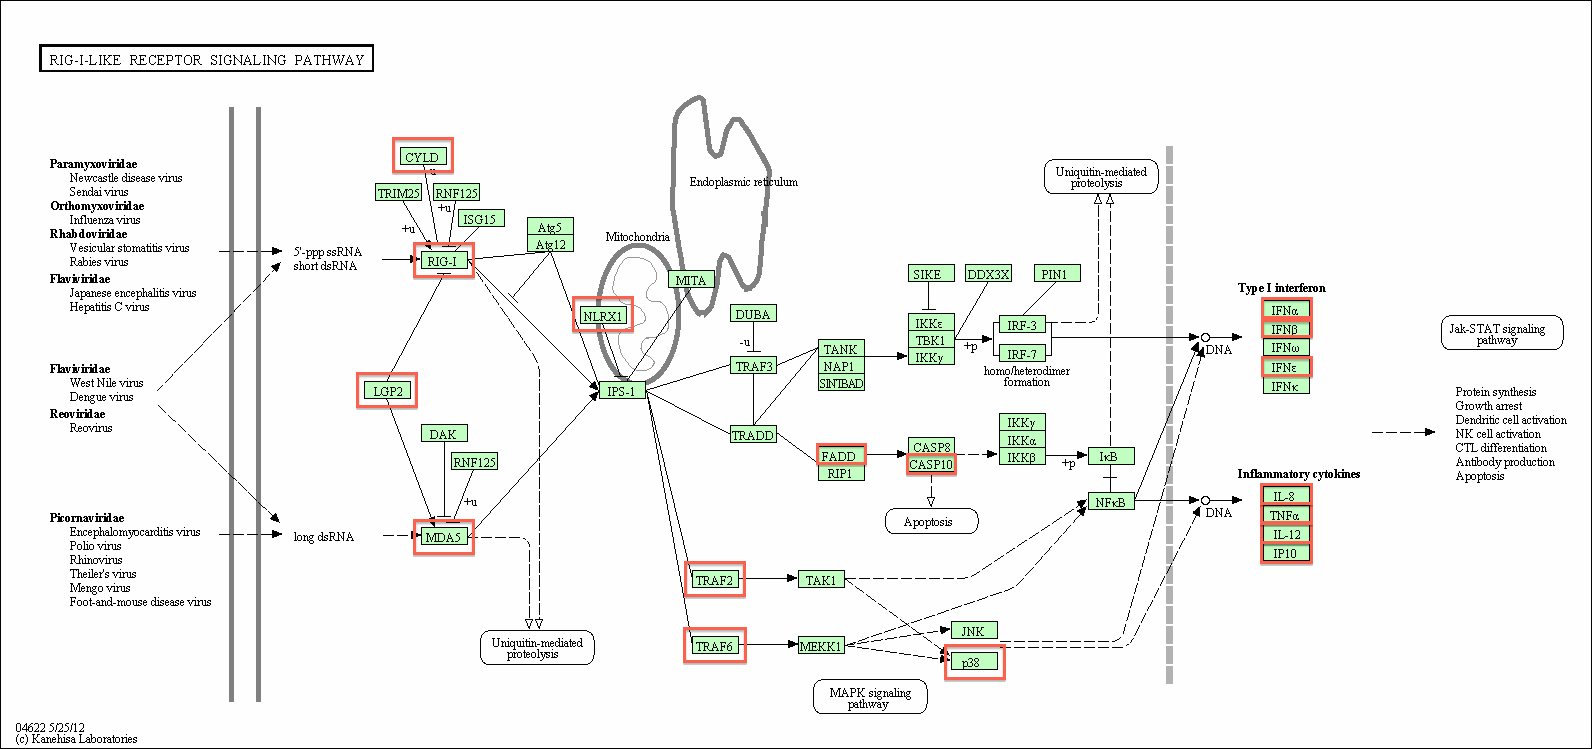
\includegraphics[width=17cm]{hsa04622.png}
\caption{RIG-I-like receptor signaling pathway for Homo sapiens with differentially expressed genes highlighted.}
\label{pathway}
\end{center}
\end{figure}


\section*{Part II: Examine Cross-Species Conservation of Pathway Genes}
% Discuss the limitations of the study and any obstacles/problems you experienced. 
% Discuss the relevance of the pathway to H5N1 infection. 
% Discuss why the conservation of the affected pathway might be important for the study of H5N1 (Hint: think about our use of model organisms to study infectious diseases). (20 points)

I studied the conservation of genes among Humans (\emph{Homo sapiens}), Mice (\emph{Mus musculus}), and Chimpanzees (\emph{Pan troglodytes}).

Instead of taking the ``RIG-I-like receptor pathway'' genes listed in the ``KEGG Pathway Genes'' text file, I decided to go back to the KEGG website \footnote{\url{http://www.kegg.jp/dbget-bin/www_bget?hsa04622}} to find the genes in the pathway for each species that I focused on. I relied on the KEGG API to search for and parse the right page to extract the list of genes.

I decided to disregard the list that was in the file given because I found that some of the ``genes'' listed for my pathway did not correspond to any human gene. Two were cDNA clones (AW511634 and AI423557), a partial CDS for a transcription factor (U88316), and another was from HeLa cells (U56433). Thus, I decided that this was not a list of human genes and went straight to the source (KEGG) for the list of genes to study. 

Additionally, I came across a duplicate gene, but under difference names. There is a gene CR936771 in my list in the KEGG pathways file that when I look up, gives me SIKE1, which is already in my list, but it is listed as SIKE, but SIKE1 is the official gene name, according to HGNC. 

\begin{figure}[ht]
\begin{center}
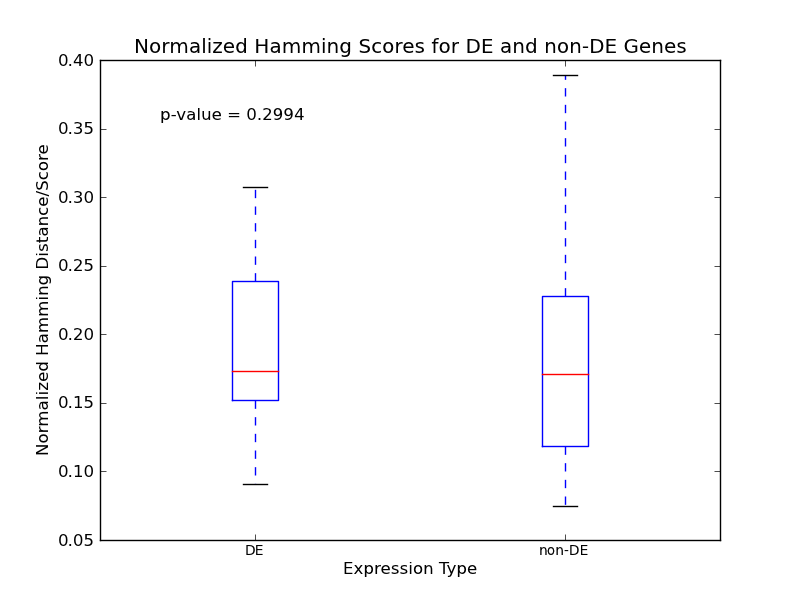
\includegraphics[width=12cm]{boxplot.png}
\caption{Boxplot of normalized Hamming distances for differentially expressed and non-differentially expressed genes in the RIG-I-like receptor pathway for Humans (\emph{Homo sapiens}), Mice (\emph{Mus musculus}), and Chimpanzees (\emph{Pan troglodytes}).\label{boxplot}}
\end{center}
\end{figure}

The decision to go to the KEGG database for the list of genes to study resulted in eighteen genes from the ``KEGG Pathway Genes'' file not being found for my pathway. As it was mentioned earlier, I found that I wouldn't have been able to find legitimate genes for five ``genes''. Thus, I did not search for thirteen genes. This may have had an effect on the final analysis. However, as you will see in the end, these thirteen missing genes must have had radical differences in them to change the overall statistical test.

I wanted to only compared genes that existed among all three species. This makes analysis easier instead of having to make a separate analysis for a pair of genes and all three genes.

We found there was no significant difference between differentially expressed genes and non-differentially expressed genes in terms of Hamming distance among three different species (p-value $= 0.2994 > 0.05$).

\section*{H5N1 Infection}

\end{document}